\documentclass[portrait]{a0poster}
\usepackage[fontsize=32pt]{fontsize}
\usepackage[bottom=3cm, left=5cm, right=5cm, a0paper]{geometry}

\newcommand{\Mateus}[1]{\textcolor{red}{[M: {\sl#1}]}}

\usepackage{hyperref}
\usepackage{float}
\usepackage{tikz}
\usepackage{paracol}
\usepackage{indentfirst}
\columnsep=60pt % spacing between columns
\columnseprule=0pt % vertical line between columns

\usepackage{physics}

\title{An Example Title for a Poster in VeryHuge Font}

\usepackage{authblk}

\author[1]{\normalsize{$^*$Mateus Marques}}
\author[2]{\normalsize{Bruno Max de Souza Melo}}
\author[3]{\normalsize{Alexandre Reily Rocha}}
\author[2]{\normalsize{Caio Lewenkopf}}
\author[1]{\normalsize{Luis G. G. V. Dias da Silva}}
\affil[1]{\textit{\small{Instituto de Física, Universidade de São Paulo, São Paulo, SP, Brazil}}}
\affil[2]{\textit{\small{Instituto de Física, Universidade Federal Fluminense, Niterói, RJ, Brazil}}}
\affil[3]{\textit{\small{Instituto de Física Teórica, São Paulo State University (UNESP), São Paulo, SP, Brazil}}}

\newcommand{\n}{\medskip}

% ------------ PARACOL SETTINGS ------------ %
\globalcounter{section}
\globalcounter{figure}
\globalcounter{table}
\setcolumnwidth{0.5\textwidth, 0.5\textwidth}
\setlength\columnsep{100pt}
\setlength{\columnseprule}{1.0pt}
% ------------------------------------------ %

%%%%%%%%%%%%%%%%%%%%%%%%%%%%%%%%%%%%%%%%%%%%%%%%%%%%%%%%%%%%%%%%%%%%%%%%%%%%%%%%

\begin{document}

%%%%%%% HEADER %%%%%%%
\tikz[remember picture, overlay] {%
%\node[rectangle, fill=#1, anchor=north, minimum width=\paperwidth, minimum height=3.5cm](header) at (current page.north){};%
\node[anchor=north, inner sep=0](header) at (current page.north){
\includegraphics[height=15cm, width=\paperwidth]{white.png}};%
\node[draw=none, align=left](description1) at ([yshift=3cm]header) { {\LARGE Charge density signatures of the Mott transition in the } };
\node[draw=none, below](description2) at (description1.south) { {\LARGE particle-hole asymmetric Hubbard model at finite temperatures} };
\node[draw=none, below](authors) at ([yshift=-1.0cm]description2.south)
{ {\large $^*$Mateus Marques$^1$, Bruno Max de Souza Melo$^2$, Alexandre Reily Rocha$^3$, Caio Lewenkopf$^2$, Luis G. G. V. Dias da Silva$^1$} };
\node[draw=none, below](affil1) at (authors.south) { { \textit{$^1$Instituto de Física, Universidade de São Paulo, São Paulo, SP, Brazil}} };
\node[draw=none, below](affil2) at (affil1.south) { { \textit{$^2$Instituto de Física, Universidade Federal Fluminense, Niterói, RJ, Brazil}} };
\node[draw=none, below](affil3) at (affil2.south) { { \textit{$^3$Instituto de Física Teórica, São Paulo State University (UNESP), São Paulo, SP, Brazil}} };
\node[draw=none, align=left](ifusp)  at ([xshift=+10cm,yshift=+2.2cm]header.west) { 
\includegraphics[height=5cm]{ifusp.png} };
\node[draw=none, align=left](fapesp) at ([xshift=-10cm,yshift=+2.2cm]header.east) { 
\includegraphics[height=3.5cm]{fapesp.png} };
}

\n\n\n\n\n

\begin{paracol}{2}
\large

\vspace{-2.0em}

\section{Introduction}

The single-band Hubbard model (SBHM) is a fundamental lattice model that accounts for electron-electron correlations, yet lacks an analytical solution for general lattices. It features the Mott transition phenomenon, which interfaces a metal (M) and an insulating (I) phase driven by the Coulomb interaction $U$. In this work, we revisit the SBHM focusing on the particle-hole asymmetric case ($\epsilon_d \neq -U/2$) at finite temperatures. We explore the limit of infinite coordination $z\to\infty$ on the Bethe lattice using the Dynamical Mean-Field Theory (DMFT) framework, with the Non-Crossing Approximation (NCA) as the impurity solver \cite{impurity-solvers}.

\vspace{-0.5em}
\section{Methods}

In second quantization, the SBHM reads
\begin{equation}
\hat{H} = \epsilon_d \sum_{i, \sigma} n_{i \sigma} + U \sum_{i } n_{i \uparrow} n_{i \downarrow} + t \sum_{\langle ij \rangle, \sigma} (c_{i \sigma }^{\dagger} c_{j \sigma} + c_{j \sigma }^{\dagger} c_{i \sigma}).
\label{eq:Hubbard_model}
\end{equation}
%\LUIS{Notice that the onsite energy term is $\epsilon_d=U/2 - \mu$ such that $\mu$ is the chemical potential $\left(\mu - U/2 \right)$}

Our study focuses on the electronic spectral function $\rho(\omega)$ and on the single-electron density $n$ given by
\begin{equation}
n = \int_{-\infty}^{\infty} \frac{\rho(\omega)}{e^{\omega/k_B T} + 1} \dd{\omega}.
\end{equation}

We use dynamical mean field theory (DMFT) \cite{georges1996} to obtain the local single-particle Green's function in momentum space $G_{\text{loc}}(\omega)$ and its spectral function $\rho(\omega)=(-1/\pi) \, \text{Im} \, \{G_{\text{loc}}(\omega)\}$. Essentially, DMFT maps a lattice many-body problem onto an auxiliary single-impurity problem through a self-consistent cycle. In the case of the SBHM, this approach simplifies to solving the single impurity Anderson model (SIAM).

We consider the Bethe lattice in the limit of infinite coordination ($z \to \infty$), where the hopping is renormalized as $t = t_*/\sqrt{z}$. In this setup, the hybridization function takes the simple form
\begin{equation}
\Delta(\omega)=t_*^2G_{\text{loc}}(\omega),
\end{equation}
and can be calculated self-consistently by iteratively applying an impurity solver. We opted for the non-crossing approximation (NCA) because of its low computational cost and effective performance at finite-temperatures. This choice enabled us to explore a wide range of parameters and capture the qualitative features of the asymmetric model for $T > 0$.

\vspace{-0.5em}
\section{Results}
\vspace{-1.5em}
\begin{figure}[H]
\centering
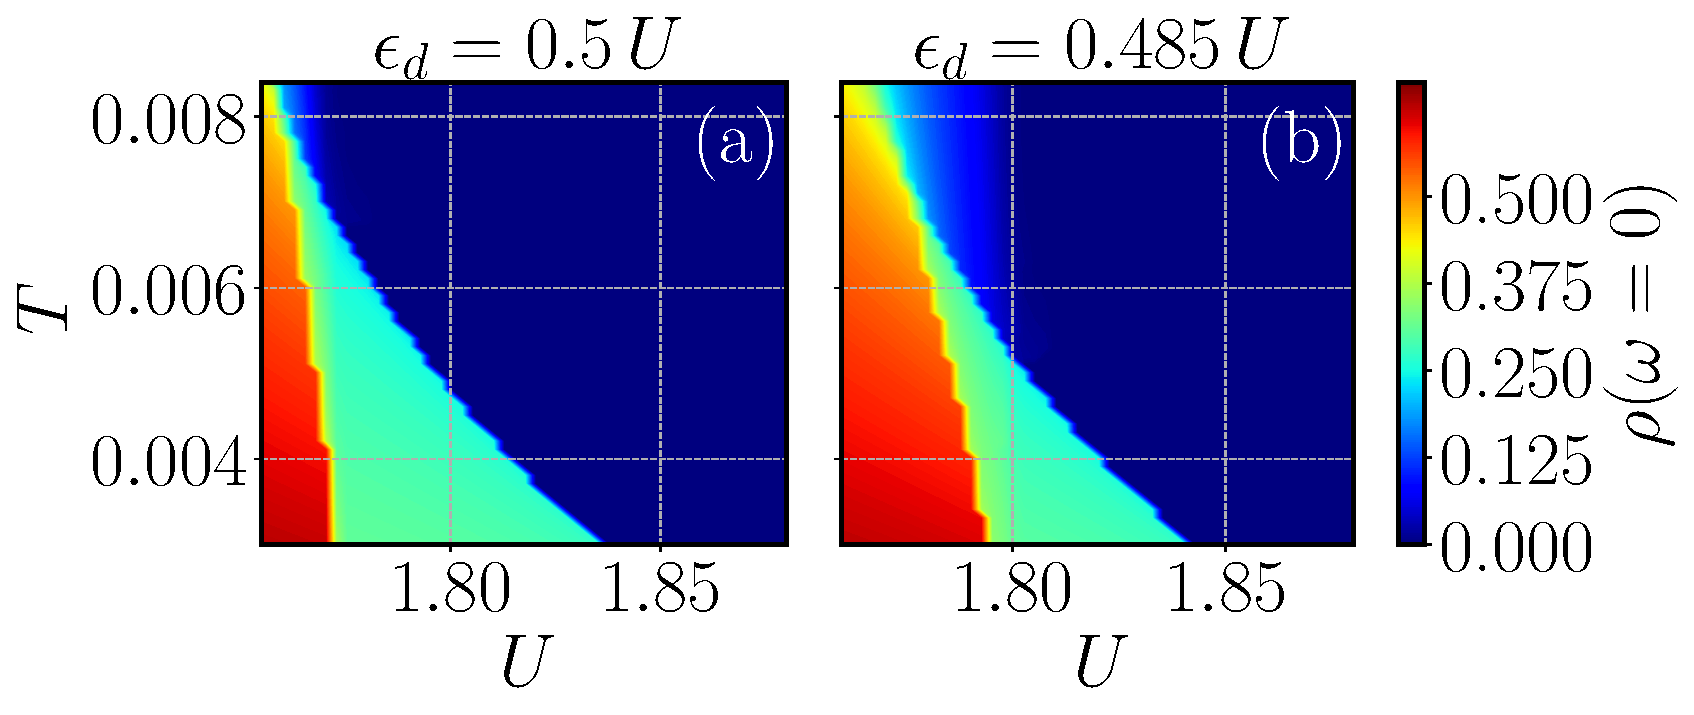
\includegraphics[width=0.8\columnwidth]{Figs/fig2-ab-eps-converted-to.pdf}
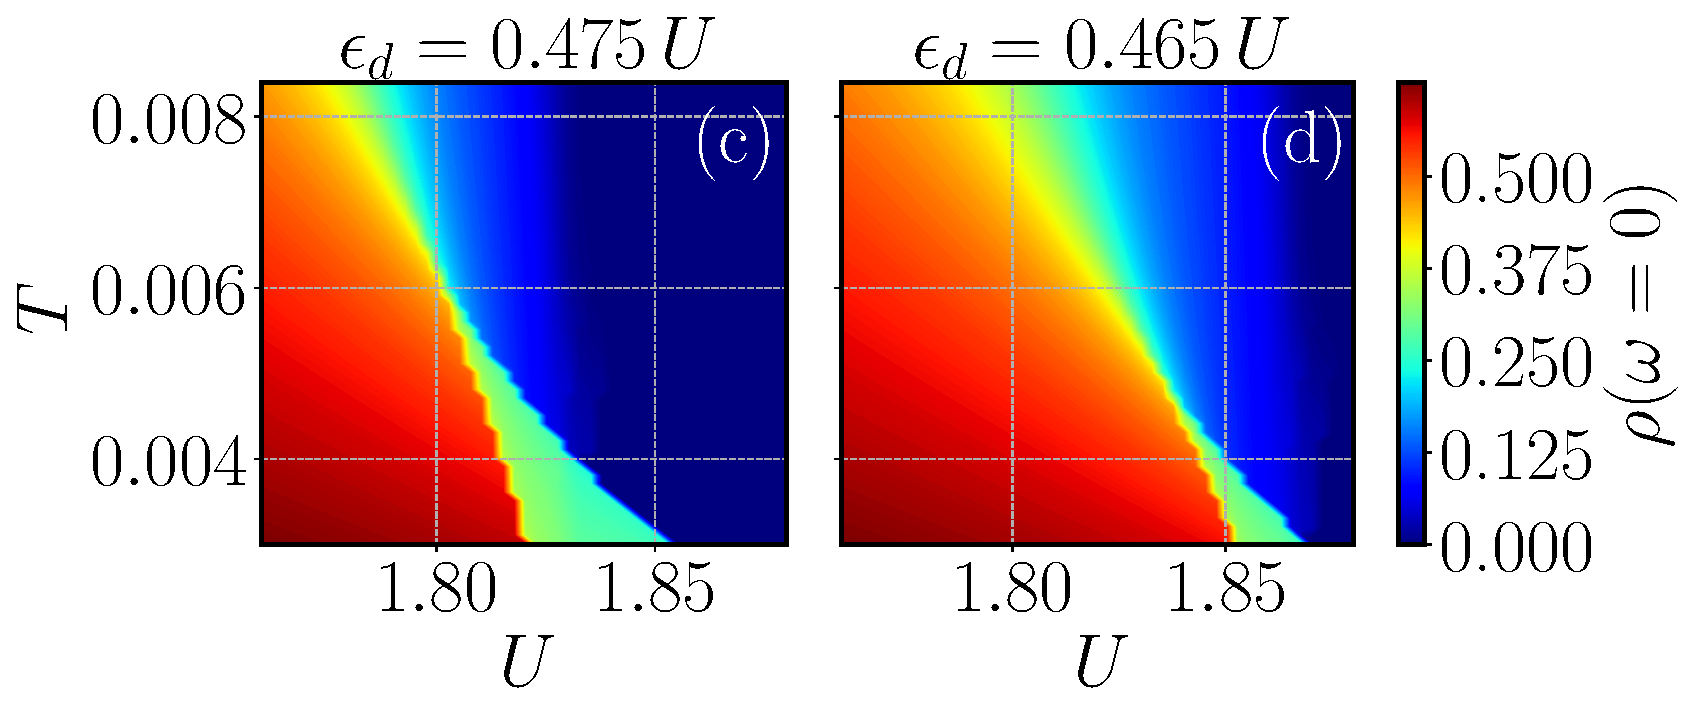
\includegraphics[width=0.8\columnwidth]{Figs/fig2-cd-eps-converted-to.pdf}
\vspace{-1em}
\caption{(a-d) SBHM phase diagrams  $U \times T$ as it is moved away from PHS. (a) $\epsilon_d=0.5U$ (PHS) (b) $\epsilon_d=0.485U$ (c) $\epsilon_d=0.475U$ (d) $\epsilon_d=0.465U$. The coexistence region (in green) shrinks as one moves away from PHS.  }
%\vspace{-10pt}
\label{fig:TvsU_ed_Tcvsed}
\end{figure}


\switchcolumn
\vspace{-0.0em}

\begin{figure}[H]
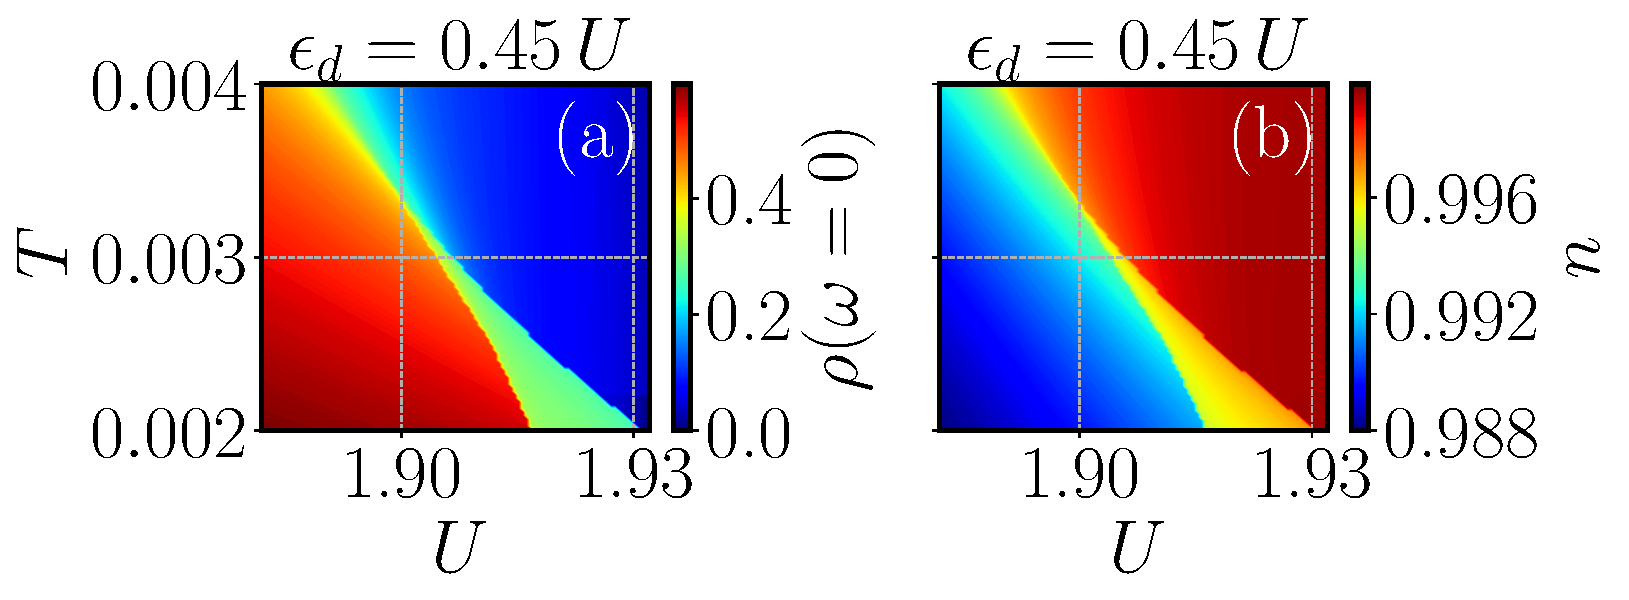
\includegraphics[width=\columnwidth]{Figs/fig3-045-eps-converted-to.pdf}
%\label{fig:Axw0T0025}
\vspace{-2em}
\caption{SBHM phase diagrams $U \times T$ away from half-filling ($\epsilon_d=0.45U$). Panel (a) shows the average spectral function $\rho(0) = (\rho_{\text{metal}}(0) + \rho_{\text{insul}}(0)) / 2$, while panel (b) shows the average density $n$.}
\label{fig:Diagram_UxT_ed045}
\end{figure}

\vspace{-1.5em}
\begin{figure}[H]
\centering
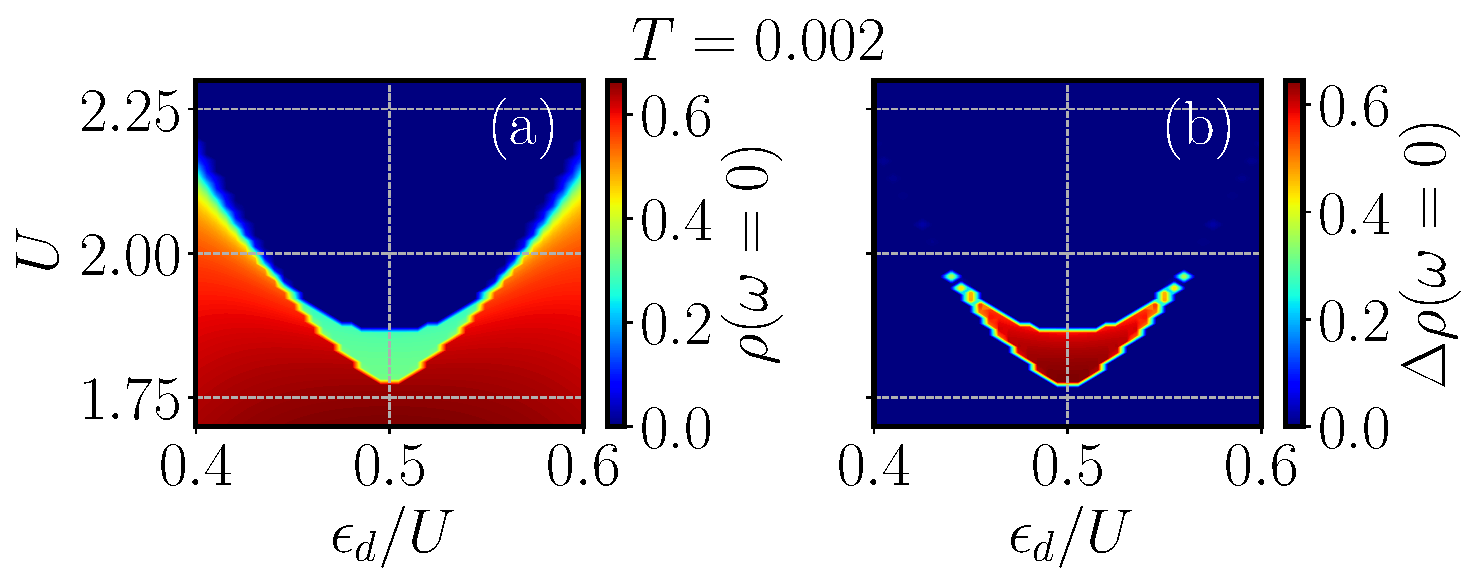
\includegraphics[width=\columnwidth]{Figs/fig4-ab-eps-converted-to.pdf}
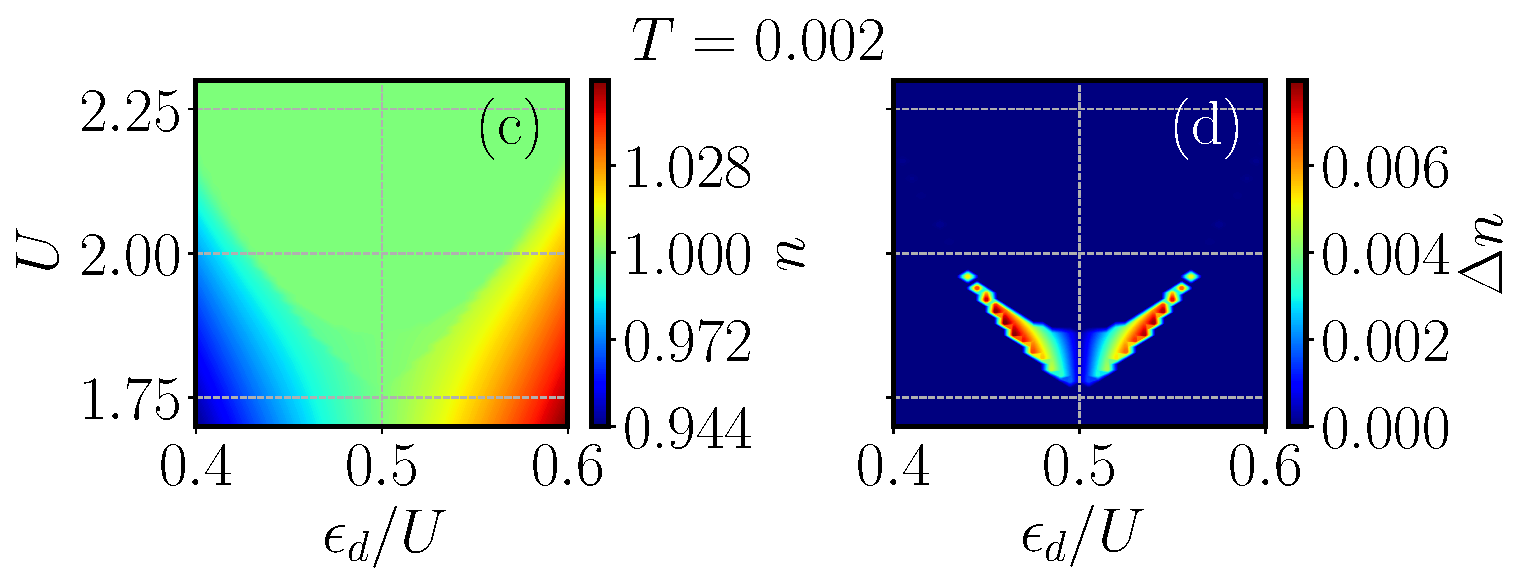
\includegraphics[width=\columnwidth]{Figs/fig5-ab-eps-converted-to.pdf}
\vspace{-1.5em}
\caption{SBHM phase diagrams $U \times \epsilon_d$ for $T=0.002$. Panels (a,b) show the avg. $(\text{M}+\text{I})/2$ and diff. $\text{M}-\text{I}$ for $\rho(0)$, and (c,d) show the avg. and diff. for $n$. }
\label{fig:Diagram_Drho_U_ed_T0002_T0004}
\end{figure}

\vspace{-1.5em}
\section{Conclusions \& Discussion}

\vspace{-0.5em}

Away from particle-hole symmetry (PHS), the Mott transition can occur as long as the filling $n$ of the system approaches one electron per site, because this is a necessary condition for the existence of an insulating phase. While earlier studies have addressed this point at zero temperature \cite{logan2015}, here we show that the system has a rich phase diagram at non-zero temperatures. More importantly, we also show that the charge density can be a reliable marker of the true Mott transition for relatively large temperatures, introducing the interesting prospect of experimentally characterizing the Mott transition by the electron (or hole) densities.

\vspace{-0.5em}
\normalsize
\bibliography{citations}
\bibliographystyle{ieeetr}

\section*{Acknowledgements}
This work is supported by the São Paulo Research Foundation (FAPESP) Grant \texttt{\#2023/02913-5}.

\end{paracol}

\end{document}
